\PassOptionsToPackage{unicode=true}{hyperref} % options for packages loaded elsewhere
\PassOptionsToPackage{hyphens}{url}
%
\documentclass[
  ignorenonframetext,
]{beamer}
\usepackage{pgfpages}
\setbeamertemplate{caption}[numbered]
\setbeamertemplate{caption label separator}{: }
\setbeamercolor{caption name}{fg=normal text.fg}
\beamertemplatenavigationsymbolsempty
% Prevent slide breaks in the middle of a paragraph:
\widowpenalties 1 10000
\raggedbottom
\setbeamertemplate{part page}{
  \centering
  \begin{beamercolorbox}[sep=16pt,center]{part title}
    \usebeamerfont{part title}\insertpart\par
  \end{beamercolorbox}
}
\setbeamertemplate{section page}{
  \centering
  \begin{beamercolorbox}[sep=12pt,center]{part title}
    \usebeamerfont{section title}\insertsection\par
  \end{beamercolorbox}
}
\setbeamertemplate{subsection page}{
  \centering
  \begin{beamercolorbox}[sep=8pt,center]{part title}
    \usebeamerfont{subsection title}\insertsubsection\par
  \end{beamercolorbox}
}
\AtBeginPart{
  \frame{\partpage}
}
\AtBeginSection{
  \ifbibliography
  \else
    \frame{\sectionpage}
  \fi
}
\AtBeginSubsection{
  \frame{\subsectionpage}
}
\usepackage{lmodern}
\usepackage{amssymb,amsmath}
\usepackage{ifxetex,ifluatex}
\ifnum 0\ifxetex 1\fi\ifluatex 1\fi=0 % if pdftex
  \usepackage[T1]{fontenc}
  \usepackage[utf8]{inputenc}
  \usepackage{textcomp} % provides euro and other symbols
\else % if luatex or xelatex
  \usepackage{unicode-math}
  \defaultfontfeatures{Scale=MatchLowercase}
  \defaultfontfeatures[\rmfamily]{Ligatures=TeX,Scale=1}
\fi
% use upquote if available, for straight quotes in verbatim environments
\IfFileExists{upquote.sty}{\usepackage{upquote}}{}
\IfFileExists{microtype.sty}{% use microtype if available
  \usepackage[]{microtype}
  \UseMicrotypeSet[protrusion]{basicmath} % disable protrusion for tt fonts
}{}
\makeatletter
\@ifundefined{KOMAClassName}{% if non-KOMA class
  \IfFileExists{parskip.sty}{%
    \usepackage{parskip}
  }{% else
    \setlength{\parindent}{0pt}
    \setlength{\parskip}{6pt plus 2pt minus 1pt}}
}{% if KOMA class
  \KOMAoptions{parskip=half}}
\makeatother
\usepackage{xcolor}
\IfFileExists{xurl.sty}{\usepackage{xurl}}{} % add URL line breaks if available
\IfFileExists{bookmark.sty}{\usepackage{bookmark}}{\usepackage{hyperref}}
\hypersetup{
  pdftitle={OpenStreetMap Download},
  pdfauthor={Jan-Philipp Kolb},
  pdfborder={0 0 0},
  breaklinks=true}
\urlstyle{same}  % don't use monospace font for urls
\newif\ifbibliography
\usepackage{graphicx,grffile}
\makeatletter
\def\maxwidth{\ifdim\Gin@nat@width>\linewidth\linewidth\else\Gin@nat@width\fi}
\def\maxheight{\ifdim\Gin@nat@height>\textheight\textheight\else\Gin@nat@height\fi}
\makeatother
% Scale images if necessary, so that they will not overflow the page
% margins by default, and it is still possible to overwrite the defaults
% using explicit options in \includegraphics[width, height, ...]{}
\setkeys{Gin}{width=\maxwidth,height=\maxheight,keepaspectratio}
\setlength{\emergencystretch}{3em}  % prevent overfull lines
\providecommand{\tightlist}{%
  \setlength{\itemsep}{0pt}\setlength{\parskip}{0pt}}
\setcounter{secnumdepth}{-2}

% set default figure placement to htbp
\makeatletter
\def\fps@figure{htbp}
\makeatother


\title{OpenStreetMap Download}
\author{Jan-Philipp Kolb}
\date{08 Januar, 2020}

\begin{document}
\frame{\titlepage}

\begin{frame}{\href{https://www.openstreetmap.org/}{Download from
OpenStreetMap}}
\protect\hypertarget{download-from-openstreetmap}{}

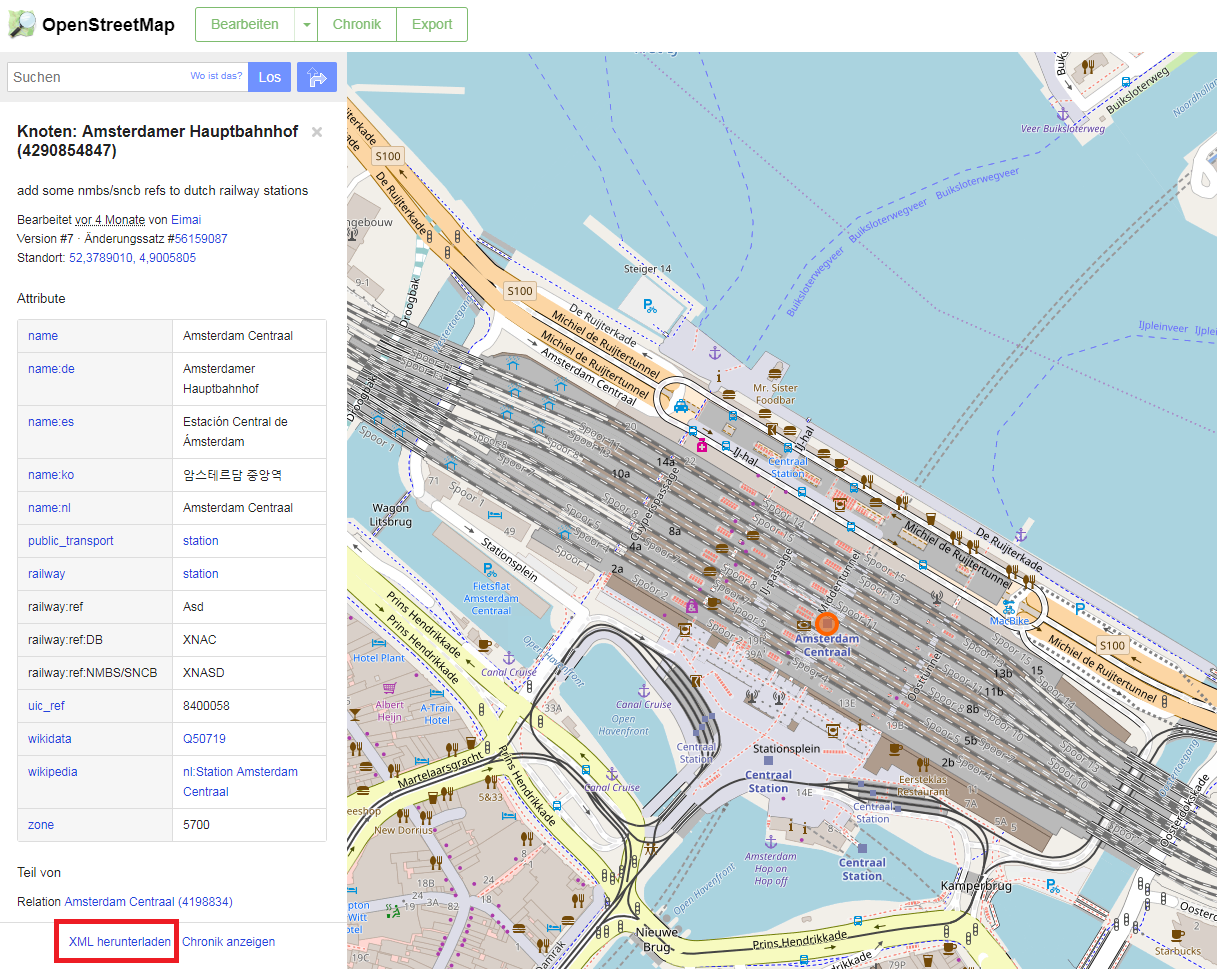
\includegraphics{figure/DownloadAmsterdamCentraal.PNG}

\end{frame}

\begin{frame}{Parse XML to R}
\protect\hypertarget{parse-xml-to-r}{}

\end{frame}

\begin{frame}[fragile]{See how data looks like}
\protect\hypertarget{see-how-data-looks-like}{}

\begin{verbatim}
## <?xml version="1.0" encoding="UTF-8"?>
## <osm version="0.6" generator="CGImap 0.6.0 (22862 thorn-03.openstreetmap.org)" copyright="OpenStreetMap and contributors" attribution="http://www.openstreetmap.org/copyright" license="http://opendatacommons.org/licenses/odbl/1-0/">
##   <node id="4290854847" visible="true" version="7" changeset="56159087" timestamp="2018-02-07T19:44:03Z" user="Eimai" uid="6072" lat="52.3789010" lon="4.9005805">
##     <tag k="name" v="Amsterdam Centraal"/>
##     <tag k="name:de" v="Amsterdamer Hauptbahnhof"/>
##     <tag k="name:es" v="Estación Central de Ámsterdam"/>
##     <tag k="name:ko" v="암스테르담 중앙역"/>
##     <tag k="name:nl" v="Amsterdam Centraal"/>
##     <tag k="public_transport" v="station"/>
##     <tag k="railway" v="station"/>
##     <tag k="railway:ref" v="Asd"/>
##     <tag k="railway:ref:DB" v="XNAC"/>
##     <tag k="railway:ref:NMBS/SNCB" v="XNASD"/>
##     <tag k="uic_ref" v="8400058"/>
##     <tag k="wikidata" v="Q50719"/>
##     <tag k="wikipedia" v="nl:Station Amsterdam Centraal"/>
##     <tag k="zone" v="5700"/>
##   </node>
## </osm>
## 
\end{verbatim}

\end{frame}

\begin{frame}{Download information for Amsterdam}
\protect\hypertarget{download-information-for-amsterdam}{}

\end{frame}

\begin{frame}[fragile]{Use of \texttt{xpathApply}}
\protect\hypertarget{use-of-xpathapply}{}

\begin{verbatim}
## [[1]]
## <tag k="population" v="844952"/> 
## 
## attr(,"class")
## [1] "XMLNodeSet"
\end{verbatim}

\end{frame}

\end{document}
